\documentclass[16.7pt]{jsarticle}

\usepackage{SPR}

\headerSPR
\begin{document}
	\titleSPR{\number\year}{\number\month}{\number\day}{D2}{吉田 皓太郎}
%%%%%%%%%%%%%%%%%%%%%%%%%%%%%%%%%%%%%%
	%\articleSPRabst
	%	\begin{itemize}
	%		\item =どういう事態か
	%	\end{itemize}
		
%今回のMTGの目的,何をディスカッションし,結果に何を得たいのかを決定する.※ミーティングごとに記入
	\articleSPRobj
		今回のMTGでは,局所修正を考慮したアルゴリズムを考慮し提案することを目標とする.これを踏まえて結果のディスカッションおよび,必要であれば修正・追加を行い,できれば論文投稿まで繋げたいと考えるため,その部分も併せてできればと思っている.
		

%%%%%%%%%%%%%%%%%%%%%%%%%%%%%%%%%%%%%%
% 1.前回からのノルマ
	\articleSPRitemsone
		%\begin{enumerate}
		%	\item A
		%\end{enumerate}
		
		\tableofcontents
		
		
%%%%%%%%%%%%%%%%%%%%%%%%%%%%%%%%%%%%%%
%\begin{itemize}
%	\item 新規手法について
%	\item ISFAアウトライン
%\end{itemize}
%%%%%%%%%%%%%%%%%%%%%%%%%%%%%%%%%%%%%%
% 2.具体的な成果
	\articleSPRitemstwo
	\renewcommand{\labelitemi}{$\blacktriangledown$}
	%\renewcommand{\labelitemi}{$\bigcirc$}
	\newcommand{\argmax}{\mathop{\rm arg~max}\limits}
	\newcommand{\argmin}{\mathop{\rm arg~min}\limits}
	\newcommand{\Ker}{{\rm Ker}}
	\newcommand{\rank}{{\rm rank}}
%%%%%%%%%%%%%%%%%%%%%%%%%%%%%%%%%%%%%
\section{データ周りの話について}
		\subsection{仮説}
		一般的には,十分にばらつきを持ったデータセットがあれば,回帰は誤差をほとんど持たずうまくいくはずである.今回のデータでは,パラメータのばらつきという部分は考慮しないまま学習させている.この事によって誤差が大きい所が発生していると考えられる.
		
		つまり,今回のデータによる誤差は,データの疎密性の問題であると言い換えられるのではないだろうか.この仮説について,考察を行った.
		\subsection{前提}
		今回のパラメータは,関数$ \alpha,\omega_{\eta},D $がそれぞれ,(仮定的に)ノイズを含んだ独立ガウス過程$ N(\bd{0},\bd{K} + \sigma^2 \bd{I}) $に従って出力されているとする.$ \bd{K} $はグラム行列を表しており,各成分を定義するカーネル関数$ k(\bd{x}_i,\bd{x}_j) $を設計することにより得る.
		\subsection{考察}
		まず初めに,特徴パラメータからガウス過程を用いて回帰させた際のハイパーパラメータに関する考察から行う.
				今回ガウス過程を適用する際に使用したカーネル関数は以下のように,RBF関数と線形関数を組み合わせたARD(関連度自動決定)カーネル関数である.ARD関数は,パラメータ毎に重みが変化し,評価値に対する相関度を自動的に決定することができる.
				\begin{equation}\label{eq:ARD_Kernel}
					k(\bd{x}_i,\bd{x}_j) = \theta_1 \exp \left[(\bd{x}_i - \bd{x}_j)^T  diag(\bd{\Theta}_R)^{-1}  (\bd{x}_i - \bd{x}_j) \right] + \bd{x}_i^T diag(\bd{\Theta}_L) \bd{x}_j
				\end{equation}
			ここで$ diag(\bd{\Theta}) $は,ベクトル$ \Theta $の各成分を対角成分に持つ対角行列である.ARDの場合は,$ \dim \bd{\Theta}_L = \dim \bd{\Theta}_R =  \dim \bd{x} $となる.
		
				また,今回特徴パラメータを抽出する際に用いたガウス過程のカーネル関数はRBF関数であったことから,1つの関数につき三つのパラメータ$ \theta_1,\theta_2,\sigma $を得る.
				今回得られた$ \Theta_L,\Theta_R $を表にまとめると,次の通りとなった.
		
				\begin{table}[h]
					\centering
					\begin{tabular}{|c|c|c|c|}
						\hline
						& $\alpha$ & $\omega_{\eta}$ & D        \\ \hline
						$\bd{\Theta}_{R,0}$        & 0.065274                      & 0.047916                             & 0.266596               \\ \hline
						$\bd{\Theta}_{R,1}$ & 158.2779                      & 5.668934                             & 0.286779               \\ \hline
						$\bd{\Theta}_{R,2}$ & 1                             & 318.7759                             & 1                    \\ \hline
		\end{tabular}
				\end{table}
		
				\begin{table}[h]
					\centering
					\begin{tabular}{|c|c|c|c|}
						\hline
						& $\alpha$ & $\omega_{\eta}$ & $D$       \\ \hline
						$\bd{\Theta}_{L,0}$        & $9.827\times 10^{-3}$ & $1.219\times 10^{-4}$        & $1.083\times 10^{-6}$ \\ \hline
						$\bd{\Theta}_{L,1}$ & $2.920\times 10^{1}$ & $8.416\times 10^{-3}$        & $1.420\times 10^{1}$ \\ \hline
						$\bd{\Theta}_{L,2}$ & $1.000$    & $2.732$        & $1.000$   \\ \hline
					\end{tabular}
				\end{table}
		この結果から,特に$ \omega_{\eta} $の分散に対して関連度が高いことが読み取れる.
		
		データの疎密性がデータ間の距離に対して強く相関関係にある仮定すれば,疎密性を定義することは,データ間の距離をうまく定義することに等しくなるため,データ間の距離について考える.
		今回考察した距離はチェベシェフ距離,マンハッタン距離に加え,今回は$ \alpha,\omega_{\eta},D $をそれぞれ独立の確率過程により生成されるとすることから,確率間の距離であるKL-Divergenceを,各関数毎に考察を行った.
		
		チェベシェフ距離,マンハッタン距離はそれぞれ次式で表される.
		\begin{equation}\label{eq:che_distance}
			d_c(\bd{x},\bd{y}) = \max_i \{ |x_i - y_i| \}
		\end{equation}
		\begin{equation}\label{eq:manhattan}
			d_m(\bd{x},\bd{y}) = \sum_{i=0}^{n-1} |x_i - y_i|
		\end{equation}
		また,KL-Divergenceは次式で定義される.
		
		\begin{equation}\label{eq:KL-Div}
			d(p,q) = \int_{-\infty}^{\infty} p \log \left( \frac{p}{q}\right) dx
		\end{equation}
		特に多変量正規分布の場合には
		\begin{equation}\label{eq:KL_Div2}
			\frac{1}{2} \left[ \log \frac{|\Sigma_1|}{|\Sigma_0|} -dim + Tr(\Sigma_1^{-1} \Sigma_0 ) + (\bd{\mu}_1 - \bd{\mu}_0)^T \Sigma_1^{-1} (\bd{\mu}_1 - \bd{\mu}_0)\right]
		\end{equation}
		となる.
		
		今回の数値検証では,検証データのパラメータ集合$\bd{\Phi}_t $と訓練データのパラメータ集合$ \bd{\Phi}_s $において,各検証データのパラメータ$ \bd{\phi}_{i,t} \in \bd{\Phi}_t  $に対して,データ間の距離$ d_i $を以下で定義した.
		\begin{equation}\label{eq:dist_data}
			d_i = \min_{j} d_{method}(\bd{\phi}_{i,t} , \bd{\phi}_{j,s})
		\end{equation}
	 	
		これらのデータでそれぞれまとめたものを次の図で示す.また,先ほどの議論から,$ \omega_{\eta} $の分散と誤差の分布を示す.
			\begin{figure}[h]
			\centering
			\begin{minipage}{0.45\hsize}
				\centering
				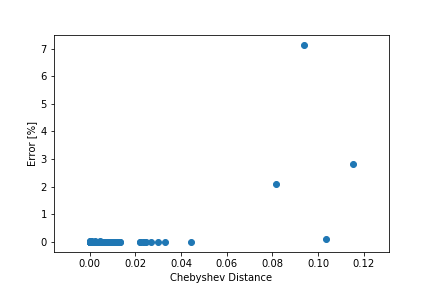
\includegraphics[width= 0.85\columnwidth]{./figure/Chebyshev.png}
				\caption{Chebyshev}
			\end{minipage}
			\begin{minipage}{0.45\hsize}
				\centering
				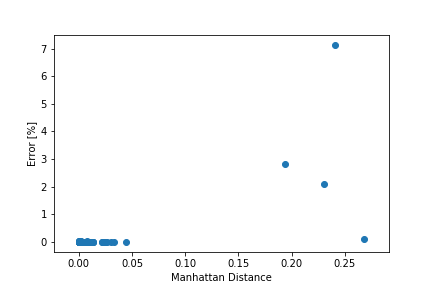
\includegraphics[width= 0.85\columnwidth]{./figure/Manhattan.png}
				\caption{Manhattan}
			\end{minipage}
		\end{figure}
		\begin{figure}[h]
			\centering
			\begin{minipage}{0.45\hsize}
				\centering
				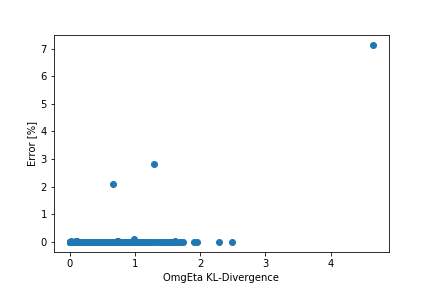
\includegraphics[width= 0.85\columnwidth]{./figure/OmgEta_Div.png}
				\caption{$ \omega_{\eta} $-KL Divergence}
			\end{minipage}
			\begin{minipage}{0.45\hsize}
				\centering
				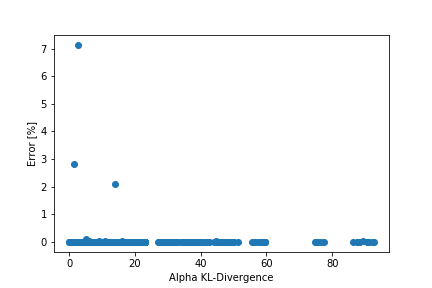
\includegraphics[width= 0.85\columnwidth]{./figure/Alpha_Div.png}
				\caption{$ \alpha $-KL Divergence}
			\end{minipage}
				\begin{minipage}{0.45\hsize}
				\centering
				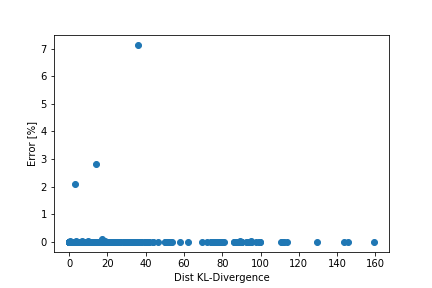
\includegraphics[width= 0.85\columnwidth]{./figure/Dist_Div.png}
				\caption{$ D $-KL Divergence}
			\end{minipage}
		\begin{minipage}{0.45\hsize}
			\centering
			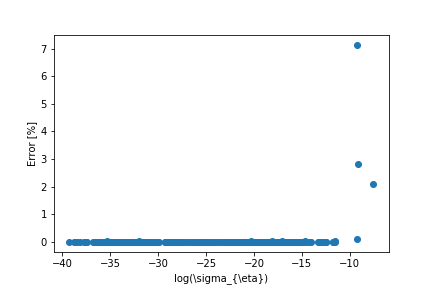
\includegraphics[width= 0.85\columnwidth]{./figure/sigma_eta.png}
			\caption{関連度高いパラメータとの相関}
		\end{minipage}
		\end{figure}
		各相関係数は以下になる.
		\begin{table}[h]
			\begin{tabular}{|c|c|c|c|c|c|c|}
				\hline
				& chebyshev & Manhattan &$\omega_{\eta}$-Divergence & $\alpha$-Divergence & $D$-Divergence & Relationship parameter \\ \hline
				相関係数 & 0.665274  & 0.72512  & 0.266596           & -0.053            & 0.0004218        & 0.474                  \\ \hline
			\end{tabular}
		\end{table}
		
		
%		まず初めに,特徴パラメータからガウス過程を用いて回帰させた際のハイパーパラメータに関する考察から行う.
%		今回ガウス過程を適用する際に使用したカーネル関数は以下のように,RBF関数と線形関数を組み合わせたARD(関連度自動決定)カーネル関数である.ARD関数は,パラメータ毎に重みが変化し,評価値に対する相関度を自動的に決定することができる.
%		\begin{equation}\label{eq:ARD_Kernel}
%			k(\bd{x}_i,\bd{x}_j) = \theta_1 \exp \left[(\bd{x}_i - \bd{x}_j)^T  diag(\bd{\Theta}_R)^{-1}  (\bd{x}_i - %\bd{x}_j) \right] + \bd{x}_i^T diag(\bd{\Theta}_L) \bd{x}_j
%		\end{equation}
%		ここで$ diag(\bd{\Theta}) $は,ベクトル$ \Theta $の各成分を対角成分に持つ対角行列である.ARDの場合は,$ \dim \bd{\Theta}_L = \dim \bd{\Theta}_R =  \dim \bd{x} $となる.
		
%		また,今回特徴パラメータを抽出する際に用いたガウス過程のカーネル関数はRBF関数であったことから,1つの関数につき三つのパラメータ$ \theta_1,\theta_2,\sigma $を得る.
%		今回得られた$ \Theta_L,\Theta_R $を表にまとめると,次の通りとなった.
		
%		\begin{table}[h]
%			\centering
%			\begin{tabular}{|c|c|c|c|}
%				\hline
%				& $\alpha$ & $\omega_{\eta}$ & D        \\ \hline
%				$\bd{\Theta}_{R,0}$        & $1.532\times 10^1$ & $2.087\times 10^1$        & $3.751\times %10^1$ \\ \hline
%				$\bd{\Theta}_{R,1}$ & $6.318\times 10^{-3}$ & $1.764\times 10^{-1}$        & $3.487\times 10^{-2}$ \\ \hline
%				$\bd{\Theta}_{R,2}$ & $1.000$    & $3.137\times 10^{-3}$        & $1.000$   \\ \hline
%			\end{tabular}
%		\end{table}
	
%		\begin{table}[h]
%			\centering
%			\begin{tabular}{|c|c|c|c|}
%				\hline
%				& $\alpha$ & $\omega_{\eta}$ & $D$       \\ \hline
%				$\bd{\Theta}_{L,0}$        & $9.827\times 10^{-3}$ & $1.219\times 10^{-4}$        & $1.083\times 10^{-6}$ \\ \hline
%				$\bd{\Theta}_{L,1}$ & $2.920\times 10^{1}$ & $8.416\times 10^{-3}$        & $1.420\times 10^{1}$ \\ \hline
%				$\bd{\Theta}_{L,2}$ & $1.000$    & $2.732$        & $1.000$   \\ \hline
%			\end{tabular}
%		\end{table}
%	$\bd{\Theta}_{R,i} (i=0,1,2)$に対するパラメータの計算オーダーは以下のようになる.
%	\begin{table}[h]
%		\centering
%		\begin{tabular}{|c|c|c|c|}
%			\hline
%			& $\alpha$ & $\omega_{\eta}$ & $D$        \\ \hline
%			$\bd{\Theta}_{L,0}$        &   $10^{-2}$& $10^{0}$        & $10^{-2}$ \\ \hline
%			$\bd{\Theta}_{L,1}$ & $ 10^{-1}$ & $10^{-1}$        & $10^{-1}$ \\ \hline
%			$\bd{\Theta}_{L,2}$ & $10^{-15}$    & $10^{-3}$        & $10^{-16}$   \\ \hline
%		\end{tabular}
%	\end{table}
%	となっている.
	
%	この事を考慮すると,$ \alpha $に対する特徴パラメータの差分に対してカーネル関数の値が他の値に対して大きく変化することが分かる.すなわち今回の評価関数は,主に$ \alpha $が支配的な要因であることが読み取れる.
	
%	仮にデータの疎密性がデータ間の距離に対して強く相関関係にあるとすれば,疎密性を定義することは,データ間の距離をうまく定義することに等しくなるため,これについて考える.
	
%	今回はデータの距離を定義するにあたって,2つの距離を用いて,$ \alpha $の特徴パラメータに対する評価誤差について考察を行った.
	
%	今回用いるパラメータは,オーダーのばらつきが大きいことから,1つ目はチェベシェフ距離を採用する.
	\section{次回のMTGについて(終了後記載)}
	\begin{itemize}
		\item  
		\item 
	\end{itemize}
	###
	\newpage
%\vspace{10cm}
%%%%%%%%%%%%%%%%%%%%%%%%%%%%%%%%%%%%%%
% 3.達成できなかったこととその問題点
	%\articleSPRthree
	
%%%%%%%%%%%%%%%%%%%%%%%%%%%%%%%%%%%%%%

%\vspace{14cm}
%%%%%%%%%%%%%%%%%%%%%%%%%%%%%%%%%%%%%%
	%\articleSPRfour
	%\articleSPRfive
\end{document}
